\documentclass[UTF8]{ctexart}
\usepackage{siunitx}
\usepackage{tikz,times,amsmath}
\usepackage{xcolor}
\usepackage{tikz-3dplot}
\usetikzlibrary{patterns}
\usetikzlibrary{positioning} % for relative positions
\usetikzlibrary{3d,calc}

\title{Note: \\What is Tensor?}
\date{\today}
\author{Clarence}

\usepackage{hyperref}
\hypersetup{
    hidelinks,
    colorlinks = false
}

\usepackage{amsthm}
\theoremstyle{definition}
\newtheorem{definition}{Definition}[section]

\theoremstyle{remark}
\newtheorem*{note}{Note}

\begin{document}

\maketitle
\newpage

\tableofcontents
\newpage

\section{Introduction}
\label{sec:introduction}

\paragraph{Examples of tensors}
\label{par:examples_of_tensors}

\subparagraph{Example 1}
\label{subp:example_1}
Specifying temperature in NYC: \( T = 273 \mathrm{K} \). It's a \textbf{Scalar}. We need one component -- 0 basis vectors/component.(i.e. it has no directions, only magnitude)
% subparagraph Example 1 (end)

\subparagraph{Example 2}
\label{subp:example_2}
Displacement $\vec d$ from Point $A$ to Point $B$

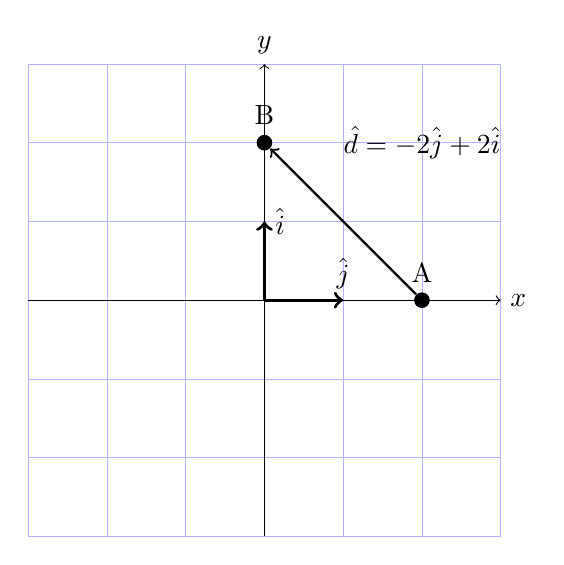
\begin{tikzpicture}[dot/.style={circle,inner sep=2pt,fill,label={#1},name=#1}]
  \draw[help lines,color=blue!30,step=1] (-3,-3) grid (3,3) ;
  \node [dot=A] at (2,0) {};
  \node [dot=B] at (0,2) {};
  \node [name=text] at (2,2) {$\hat d = -2 \hat j + 2 \hat i$};
  \draw [thick,->] (A) -- (B);
  \draw [->] (-3,0) -- (3,0) node [right]{$x$};
  \draw [->] (0,-3) -- (0,3) node [above]{$y$};
  \draw [->,very thick] (0,0) -- (0,1) node [right]{$\hat i$};
  \draw [->,very thick] (0,0) -- (1,0) node [above]{$\hat j$};
  % draw[domain =0:4] plot (\x ,{0.1* exp(\x)}) node[right] {$f(x)=\frac{1}{10}e^x$};
  % \draw [thick,->](0,2)--(2,0);
\end{tikzpicture}

$ \begin{Vmatrix} \vec{d} \end{Vmatrix} = 2\sqrt{2} \si{km}  $,
$ \vec{d} $ in direction of $ \vec{AB}$. \\
It's a \textbf{Vector}: 2 components (1 basis vector/component)
% subparagraph Example 2 (end)

\subparagraph{Example 3}
\label{subp:example_3}
Suppose looking at a rectangular steel on a bridge. Considering its stresses on Point $O$.

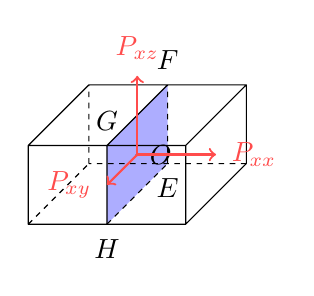
\begin{tikzpicture}[anchor=base, baseline]
\coordinate (A) at (2,0,0);
\coordinate (B) at (2,1,0);
\coordinate (C) at (0,1,0);
\coordinate (D) at (0,0,0);
\coordinate (A') at (2,0,2);
\coordinate (B') at (2,1,2);
\coordinate (C') at (0,1,2);
\coordinate (D') at (0,0,2);

\coordinate (E) at(1,0,0);
\coordinate (F) at(1,1,0);
\coordinate (G) at(1,1,2);
\coordinate (H) at(1,0,2);
\coordinate (O) at(1,0.5,1);

\fill[blue!40!white,opacity=0.8](E)--(F)--(G)--(H)--cycle;
\draw[rounded corners=0.05pt]
  (A')--(B')--(C')--(D')--(A')--cycle
  (A)--(B)--(C)
  (A')--(A)(B')--(B)(C')--(C)

  (E)node[below=2pt]{$E$}
  (O)circle (0.3pt)node[right=1pt]{$O$}

  (F)node[above=2pt]{$F$}--
  (G)node[above=2pt]{$G$}--
  (H)node[below=2pt]{$H$};
\draw[thin,dash pattern=on 2pt off 2pt]
  (D')--(D)
  (D)--(C)
  (A)--(D)
  (E)--(F)
  (H)--(E);

\draw[thick, ->, red!70] (O)--($(O)+(1,0,0)$) node[right=2pt]{$P_{xx}$};
\draw[thick, ->, red!70] (O)--($(O)+(0,1,0)$) node[above=2pt]{$P_{xz}$};
\draw[thick, ->, red!70] (O)--($(O)+(0,0,1)$) node[left=2pt]{$P_{xy}$};

\tdplotsetmaincoords{60}{45}
\end{tikzpicture}
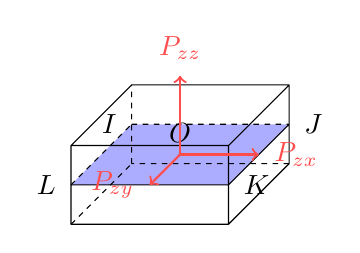
\begin{tikzpicture}[anchor=base, baseline]
\coordinate (A) at (2,0,0);
\coordinate (B) at (2,1,0);
\coordinate (C) at (0,1,0);
\coordinate (D) at (0,0,0);
\coordinate (A') at (2,0,2);
\coordinate (B') at (2,1,2);
\coordinate (C') at (0,1,2);
\coordinate (D') at (0,0,2);

\coordinate (E) at(0,0.5,0);
\coordinate (F) at(2,0.5,0);
\coordinate (G) at(2,0.5,2);
\coordinate (H) at(0,0.5,2);
\coordinate (O) at(1,0.5,1);

\fill[blue!40!white,opacity=0.8](E)--(F)--(G)--(H)--cycle;
\draw[rounded corners=0.05pt]
  (A')--(B')--(C')--(D')--(A')--cycle
  (A)--(B)--(C)
  (A')--(A)(B')--(B)(C')--(C)

  (E)node[left=2pt]{$I$}
  (O)circle (0.3pt)node[above=1pt]{$O$}

  (F)node[right=2pt]{$J$}--
  (G)node[right=2pt]{$K$}--
  (H)node[left=2pt]{$L$};

\draw[thin,dash pattern=on 2pt off 2pt]
  (D')--(D)
  (D)--(C)
  (A)--(D)
  (E)--(F)
  (H)--(E);

\draw[thick, ->, red!70] (O)--($(O)+(1,0,0)$) node[right=2pt]{$P_{zx}$};
\draw[thick, ->, red!70] (O)--($(O)+(0,1,0)$) node[above=2pt]{$P_{zz}$};
\draw[thick, ->, red!70] (O)--($(O)+(0,0,1)$) node[left=2pt]{$P_{zy}$};
\tdplotsetmaincoords{60}{45}
\end{tikzpicture}
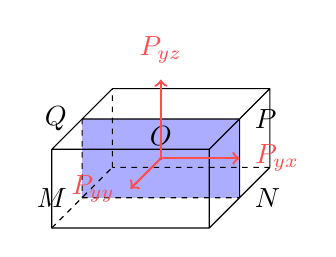
\begin{tikzpicture}[anchor=base, baseline]
\coordinate (A) at (2,0,0);
\coordinate (B) at (2,1,0);
\coordinate (C) at (0,1,0);
\coordinate (D) at (0,0,0);
\coordinate (A') at (2,0,2);
\coordinate (B') at (2,1,2);
\coordinate (C') at (0,1,2);
\coordinate (D') at (0,0,2);

\coordinate (E) at(0,0,1);
\coordinate (F) at(2,0,1);
\coordinate (G) at(2,1,1);
\coordinate (H) at(0,1,1);
\coordinate (O) at(1,0.5,1);

\fill[blue!40!white,opacity=0.8](E)--(F)--(G)--(H)--cycle;
\draw[rounded corners=0.05pt]
  (A')--(B')--(C')--(D')--(A')--cycle
  (A)--(B)--(C)
  (A')--(A)(B')--(B)(C')--(C)

  (E)node[left=2pt]{$M$}
  (O)circle (0.3pt)node[above=1pt]{$O$}

  (F)node[right=2pt]{$N$}--
  (G)node[right=2pt]{$P$}--
  (H)node[left=2pt]{$Q$};

\draw[thin,dash pattern=on 2pt off 2pt]
  (D')--(D)
  (D)--(C)
  (A)--(D)
  (E)--(F)
  (H)--(E);

\draw[thick, ->, red!70] (O)--($(O)+(1,0,0)$) node[right=2pt]{$P_{yx}$};
\draw[thick, ->, red!70] (O)--($(O)+(0,1,0)$) node[above=2pt]{$P_{yz}$};
\draw[thick, ->, red!70] (O)--($(O)+(0,0,1)$) node[left=2pt]{$P_{yy}$};
\tdplotsetmaincoords{60}{45}
\end{tikzpicture}

\begin{tikzpicture}
\coordinate (X) at(1,0,0);
\coordinate (Z) at(0,1,0);
\coordinate (Y) at(0,0,1);
\coordinate (O) at(0,0,0);
\draw[rounded corners=0.05pt, ->, thick]
  (O)--(X)node[right=2pt]{$\hat x$};
\draw[rounded corners=0.05pt, ->, thick]
  (O)--(Z)node[above=2pt]{$\hat z$};
\draw[rounded corners=0.05pt, ->, thick]
  (O)--(Y)node[left=2pt]{$\hat y$};
\tdplotsetmaincoords{60}{45}
\end{tikzpicture}

In these diagrams, take $ P_{xy} $ as an example, the subscript x means the cross-sectional area of the force is perpendicular to $ \hat x $, and the subscript $ \hat y $ indicates the direction of the force.

We can actually combine all these forces per unit area components into a $ 3 \times 3 $ matrix as follows:

\[
P =
\begin{bmatrix}
  P_{xx} & P_{xy} & P_{xz} \\
  P_{yx} & P_{yy} & P_{yz} \\
  P_{zx} & P_{zy} & P_{zz} \\
\end{bmatrix}
.\]
Why don't we just add the forces in the same direction and just end up as a force per unit area \textbf{Vector} instead of a \textbf{matrix}?

For example, why don't we just add up $ P_{xx} $ and $ P_{yx} $? After all, they are acting in the same $ \hat x $ direction.
It's because even though they are acting in the same direction on the same point, the nature of those forces is different. $ P_{xx} $ pulls the Point $ O $ forward, and $ P_{xy} $ shears/drags $O$ forward. They cause the steel to form in different ways. That's why in addition to specifying the force, it's necessary to specify the surface the force is acting on.

So we use $P$, which is a matrix that has 9 components, and each component is specified by a magnitude and 2 basis vectors, 1 vector for the cross-sectional area that is being acted on,
the other vector for the force acting on that area.

% subparagraph Example 3 (end)

% paragraph Examples of tensors (end)

Actually all these 3 mathematical objects have something in common. They are all \textbf{Tensors}.

\begin{definition}[Tensor]
  In an $m$-dimensional space, a tensor of rank $n$, is a mathematical object that has $n$ indices, $m^n$ components and \textbf{obey certain transformation rules}. (Generally $n = 3$, one exception is General Relativity, where we use 4 dimensions,with time being an additional dimension)
\end{definition}
Having to pointed out that matrix is not accurately equivalent to a tensor of rank 2. A matrix is just a bunch of numbers, and tensor must obey some transformation rules.
\begin{note}[Rank of Tensor]
  Number of basis vectors needed to fully specify a component of the tensor.
\end{note}

% section Introduction (end)

\section{Transformation Rules}
\label{sec:transformation_rules}
There are actually 2 ways to describe the transformation rules of tensors.
Physicists especially love the first description:
\begin{itemize}
  \item A tensor is a mathematical object that transforms like a tensor.
\end{itemize}
The more helpful one is:
\begin{itemize}
  \item A tensor is an object that is invariant under a change of a coordinate systems. When we do change the coordinate systems, the components change according to a special set of mathematical rules.
\end{itemize}

The first way to describe tensor is ridiculously bad of beginners, that's why we are going to use the second way to describe the transformation rules of tensors.
In order to do that, let's go back to the tensors discussed before.

Obviously, no matter what coordinate system we choose, the temperature $T$ will not change. It's a scalar.

Going to our displacement vector. Each of its component need 1 basis vector to be described, so a displacement vector is a tensor of rank 1.

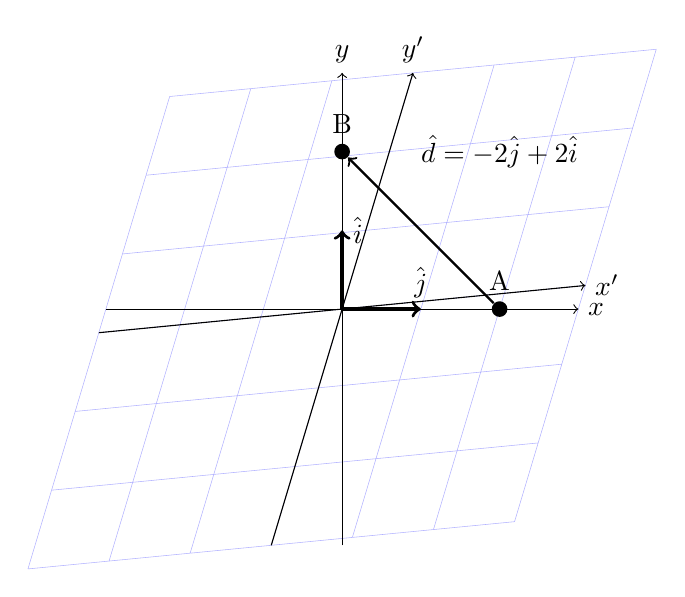
\begin{tikzpicture}[dot/.style={circle,inner sep=2pt,fill,label={#1},name=#1}]
\draw[help lines,color=blue!30,step=1,xslant=0.3,yslant=0.1] (-3,-3) grid (3,3) ;
\node[dot=A] at (2,0) {};
\node[dot=B] at (0,2) {};
\node[name=text] at (2,2) {$\hat d = -2 \hat j + 2 \hat i$};
\draw[thick,->] (A) -- (B);

\draw[->] (-3,0) -- (3,0) node [right]{$x$};
\draw[->] (0,-3) -- (0,3) node [above]{$y$};

\draw[->,xslant=0.3,yslant=0.1] (-3,0) -- (3,0) node [right]{$x'$};
\draw[->,xslant=0.3,yslant=0.1] (0,-3) -- (0,3) node [above]{$y'$};

\draw[->,very thick] (0,0) -- (0,1) node [right]{$\hat i$};
\draw[->,very thick] (0,0) -- (1,0) node [above]{$\hat j$};
% draw[domain =0:4] plot (\x ,{0.1* exp(\x)}) node[right] {$f(x)=\frac{1}{10}e^x$};
% \draw [thick,->](0,2)--(2,0);
\end{tikzpicture}

Changing the coordinate systems does changes the way we write the vector, but it doesn't change the vector itself. In fact, no matter what coordinate we choose, the vector still points from $A$ to $B$. Thus, the vector is invariant when we change the coordinate systems.

Now let's go to our rank 2 tensor: stress tensor $P$. Obviously, the choice of the coordinate system doesn't change the forces. The manner we write to express the tensor changes, but the tensor itself doesn't change.
% section Transformation Rules (end)
\end{document}
